\documentclass[conference]{IEEEtran}
\IEEEoverridecommandlockouts
% The preceding line is only needed toy funding in the first footnote. If that is unneeded, please comment it out.
\usepackage{cite}
\usepackage{amsmath,amssymb,amsfonts}
\usepackage{algorithmic}
\usepackage{graphicx}
\usepackage{textcomp}
\usepackage{xcolor}
\usepackage{booktabs}

\def\BibTeX{{\rm B\kern-.05em{\sc i\kern-.025em b}\kern-.08em
    T\kern-.1667em\lower.7ex\hbox{E}\kern-.125emX}}
\begin{document}

\title{Conference Paper Title*\\
{\footnotesize \textsuperscript{*}Note: Sub-titles are not captured in Xplore and
should not be used}

}

\author{\IEEEauthorblockN{1\textsuperscript{st} José Raimundo Alves dos Santos Júnior}
\IEEEauthorblockA{\textit{dept. name of organization (of Aff.)} \\
\textit{name of organization (of Aff.)}\\
City, Country \\
email address or ORCID}
\and
\IEEEauthorblockN{2\textsuperscript{nd} Eduardo Furtado de Simas Filho}
\IEEEauthorblockA{\textit{dept. name of organization (of Aff.)} \\
\textit{name of organization (of Aff.)}\\
City, Country \\
email address or ORCID}

}

\maketitle

\begin{abstract}
This document is a model and instructions for \LaTeX.
This and the IEEEtran.cls file define the components of your paper [title, text, heads, etc.]. *CRITICAL: Do Not Use Symbols, Special Characters, Footnotes, 
or Math in Paper Title or Abstract.
\end{abstract}

\begin{IEEEkeywords}
component, formatting, style, styling, insert
\end{IEEEkeywords}

\section{Introdução}
O monitoramento de progresso é um dos elos fundamentais para gestão de projetos, auxiliando na conclusão bem sucedida da construção de edificações e infraestruturas \cite{Pal2023}. Na construção de Obras de Arte Especiais (OAE), como as pontes, as condições diferem significativamente das edificações convencionais, caracterizando-se por processos altamente setorizados, distribuição espacial discreta e uso intensivo de componentes pré-fabricados \cite{Zhang2025}. Embora essas estruturas apresentem padrões geométricos repetitivos e similares, a extensão do canteiro e a complexidade logística impõem desafios severos à gestão e ao acompanhamento físico do projeto \cite{Zhang2025}.

Os métodos tradicionais de monitoramento do progresso se baseiam em registros manuais, inspeções \textit{in loco} e atualizações em planilhas ou papel \cite{Pal2023}. Nesse sentido, essa abordagem apresenta desvantagens críticas: é excessivamente lenta, trabalhosa, propensa a erros humanos e influenciada pela subjetividade dos inspetores \cite{Qureshi2023}. Devido à incapacidade coletar dados do canteiro com alta frequência, os dados coletados ficam rapidamente desatualizados, tornando a tomada de decisão reativa e propiciando atrasos e estouros de orçamento \cite{Reja2022}. Ademais, a simples captura visual do canteiro sem processamento automatizado não soluciona o problema, pois apenas transfere o gargalo operacional do campo para o escritório.  



Nesse cenário, a integração de ferramentas como a Modelagem da Informação da Construção (BIM) a técnicas de Visão Computacional (CV) em Inteligência Artificia (IA) tem se consolidado como a via mais eficiente para o monitoramento automatizado \cite{Pal2023}. O uso de \textit{Deep Learning} permite processar dados visuais complexos, como nuvens de pontos, visando comparar o modelo planejado (\textit{as-planned}) com a execução real (\textit{as-built}) para extrair informações objetivas de avanço \cite{Reja2022,Braun2020 }.  

Apesar desses avanços, a literatura e as aplicações de monitoramento automatizado ainda concentram-se majoritariamente em edificações verticais, revelando uma lacuna no desenvolvimento de fluxos adaptados às especificidades geométricas e operacionais das pontes. Portanto, este trabalho propõe aplicar a eliminação de ruídos de nuvens de pontos utilizando \textit{deep learning} (RandLA-Net) como etapa necessária para aplicar um fluxo semi-automatizado para o monitoramento do progresso de pontes. O resultado da eliminação de ruídos terá uso em futuros algoritmos de alinhamento geométrico, visando eliminar a carga manual, fornecer dados acionáveis aos gestores e mitigar ineficiências construtivas.


\section{Revisão Bibliográfica}

\section{Descrição dos métodos utilizados}
\subsection{RandLaNET}
\subsection{Dados Utilizados}
\subsubsection{SemanticBridge}

Para o treinamento, foram utilizados os dados públicos do SemanticBridge~\cite{SemanticBridge}, disponibilizados sob a licença CC-BY-4.0. O conjunto reúne 27 nuvens de pontos de 20 pontes, adquiridas com três tecnologias de escaneamento diferentes:
\begin{itemize}
	\item \textbf{FARO} (escâner laser terrestre, TLS): 10 cenas, com distância mediana entre vizinhos de 4,0 a 5,6~cm;
	\item \textbf{Leica RTC360} (TLS): 10 cenas, com 2,3 a 2,9~cm;
	\item \textbf{Leica BLK2GO} (escâner laser móvel, MLS): 7 cenas, com 2,3 a 3,7~cm.
\end{itemize}
Todas as nuvens possuem informação de cor (RGB). Sete pontes (12, 13 e 15 a 19) foram capturadas por dois sensores (BLK2GO e RTC360), de modo que o mesmo local aparece em duas nuvens.

Cada ponto possui um rótulo binário (ponte ou ambiente), derivado das classes de componentes do conjunto. Os pontos sem rótulo, entre 0,3\% e 1,9\% de cada cena, foram ignorados no treinamento e na avaliação.

Os dados foram divididos em treinamento, validação e teste na proporção aproximada de 63\%, 18,5\% e 18,5\% das cenas (17, 5 e 5 cenas, respectivamente), conforme a Tabela~\ref{tab:divisao}. O sorteio das pontes foi estratificado por grupo de sensor (FARO e Leica), com semente fixa. O conjunto de teste contém as pontes 5 e 7 (FARO) e 13 e 20 (Leica).

\begin{table}[htbp]
	\centering
	\caption{Divisão dos dados do SemanticBridge.}
	\label{tab:divisao}
	\begin{tabular}{lccc}
		\toprule
		Conjunto & Pontes & Cenas & Proporção das cenas \\
		\midrule
		Treinamento & 12 & 17 & 63,0\% \\
		Validação   &  4 &  5 & 18,5\% \\
		Teste       &  4 &  5 & 18,5\% \\
		\bottomrule
	\end{tabular}
\end{table}

\subsubsection{Dados do Getec}
	
Os dados fazem parte do projeto de pesquisa Método automatizado para monitoramento do avanço físico de obras de infraestrutura com uso do BIM 4D e fotogrametria que está sendo conduzido pelo Grupo de Pesquisa e Extensão em Gestão e Tecnologia das Construções (GETEC) em parceria com uma concessionária de infraestrutura de grande porte, reconhecida por sua atuação abrangente em obras e serviços de transporte na América Latina.

A obra analisada localiza-se na Via Dutra (BR-116), no estado do Rio de Janeiro, abrangendo um trecho de 16 km (8 km por sentido), que inclui a construção de 93 contenções e 24 obras de arte especiais. 

\begin{figure}[htbp]
	\centering
	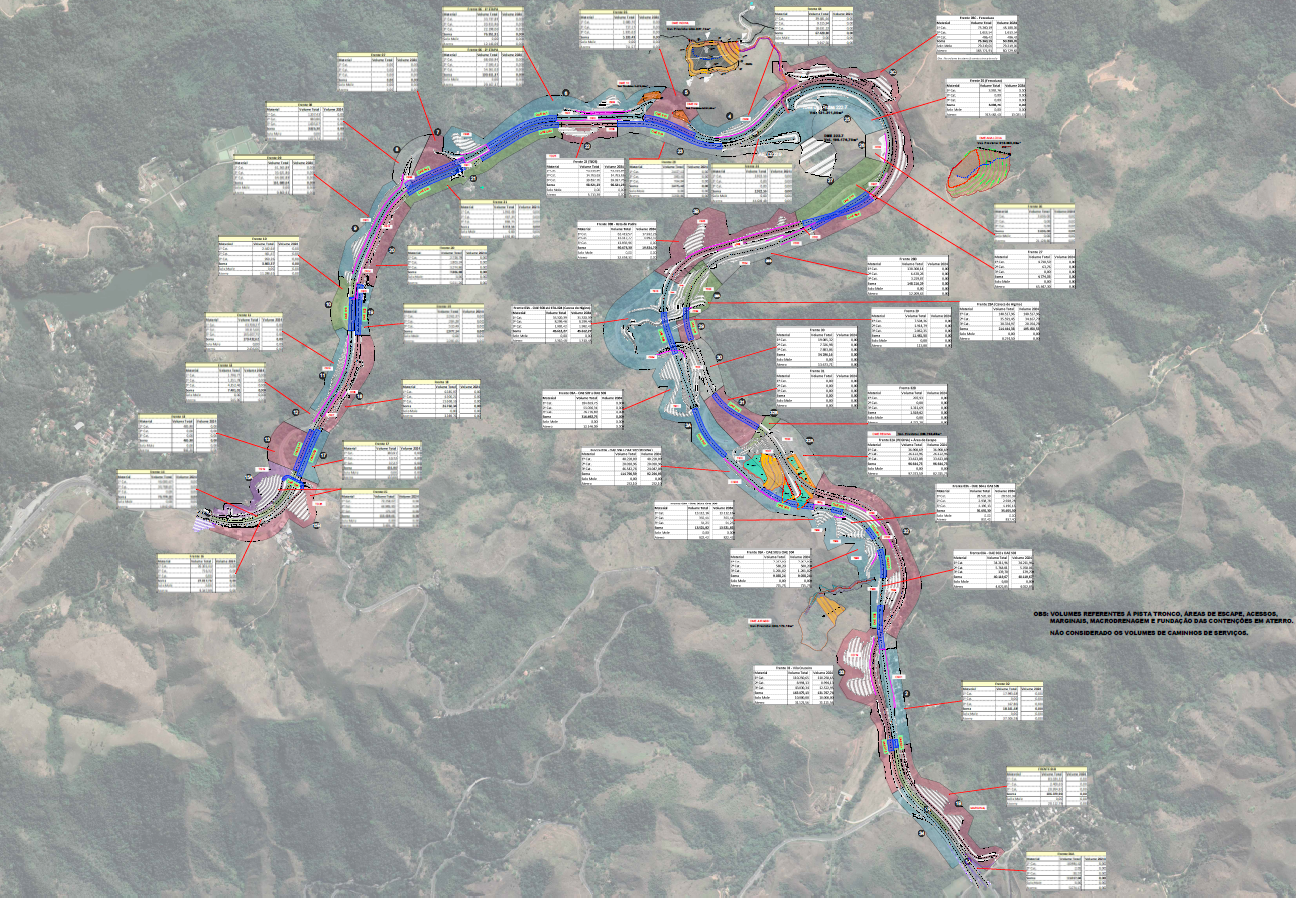
\includegraphics[width=0.45\textwidth]{figs/obra_real.png}
	\caption{Registro fotográfico da obra real.}
	\label{fig:obra_real}
\end{figure}

As Obras de Artes Especiais (OAE), escolhidas durante essa fase do projeto foram as nomeadas D19 e S07 por estarem em fases distintas de construção, permitindo discussões sobre o uso das ferramentas, parâmetros e processos em diferentes cenários. OAE D19 trata-se de um viaduto composto por 18 pilares, 67 vigas e com aproximadamente 425 m de extensão de pavimento. A OAE S07 é composta por 8 pilares, 38 vigas e com aproximadamente 222m de extensão. Neste estudo as essas OAEs foram utilizadas para validação do modelo.

\section{Resultados}

\section{Conclusão}



\begin{thebibliography}{00}

\bibitem{SemanticBridge}
	M. Kellner, M. Ferrandon Cervantes, Y. Pan, R. Lu, I. Brilakis, and A. Reiterer,
	``SemanticBridge---A dataset for 3D semantic segmentation of bridges and domain gap analysis,''
	\textit{Developments in the Built Environment},
	vol. 26, Art. no. 100912, 2026,
	doi: 10.1016/j.dibe.2026.100912.
	
\bibitem{Pal2023}
	A. Pal, J. J. Lin, S.-H. Hsieh, and M. Golparvar-Fard,
	``Automated vision-based construction progress monitoring in built environment through digital twin,''
	\textit{Developments in the Built Environment},
	vol. 16, 2023, Art. no. 100247,
	doi: 10.1016/j.dibe.2023.100247.
	
\bibitem{Zhang2025}
	H. Zhang, J. Yan, J. Yang, W. Meng, and S. Chen,
``Two-stage point cloud registration using multi-scale edge convolution for digital twin-based bridge construction progress monitoring,''
\textit{Automation in Construction},
vol. 179, Art. no. 106415, 2025,
doi: 10.1016/j.autcon.2025.106415.

\bibitem{Qureshi2023}
	A. H. Qureshi, W. S. Alaloul, W. K. Wing, S. Saad, M. A. Musarat, S. Ammad, and A. F. Kineber,
``Automated progress monitoring technological model for construction projects,''
\textit{Ain Shams Engineering Journal},
vol. 14, no. 10, Art. no. 102165, 2023,
doi: 10.1016/j.asej.2023.102165.

\bibitem{Reja2022}
V. K. Reja, K. Varghese, and Q. P. Ha,
``Computer vision-based construction progress monitoring,''
\textit{Automation in Construction},
vol. 138, Art. no. 104245, 2022,
doi: [inserir DOI].

\bibitem{Braun2020}
A. Braun, S. Tuttas, A. Borrmann, and U. Stilla,
``Improving progress monitoring by fusing point clouds, semantic data and computer vision,''
\textit{Automation in Construction},
vol. 116, Art. no. 103210, 2020,
doi: 10.1016/j.autcon.2020.103210.


\end{thebibliography}


\end{document}

